\subsection{Pipelining}

Multi-cycle processors are an improvement over single-cycles processors, but they still spend a great amount of time only doing one thing.
Pipelining is a technique that dramaticly increases the throughput of a multi-cycle processor by allowing different stages of different instructions to execute at the same time.

The execution of an instruction is usually split into five stages:
Fetch, Decode, Execute, Memory and Writeback. 
This means that 5 different instructions can be executed in parallell,
one in each stage, as seen below in figure \ref{fig:pipeline}.
\footnote{
    The number of stages can vary.
    Some versions of Intel Pentium 4 had a whopping 31-stage pipeline.
    \cite{wiki-pentium4}
}

\begin{figure}[ht]
    \centering
    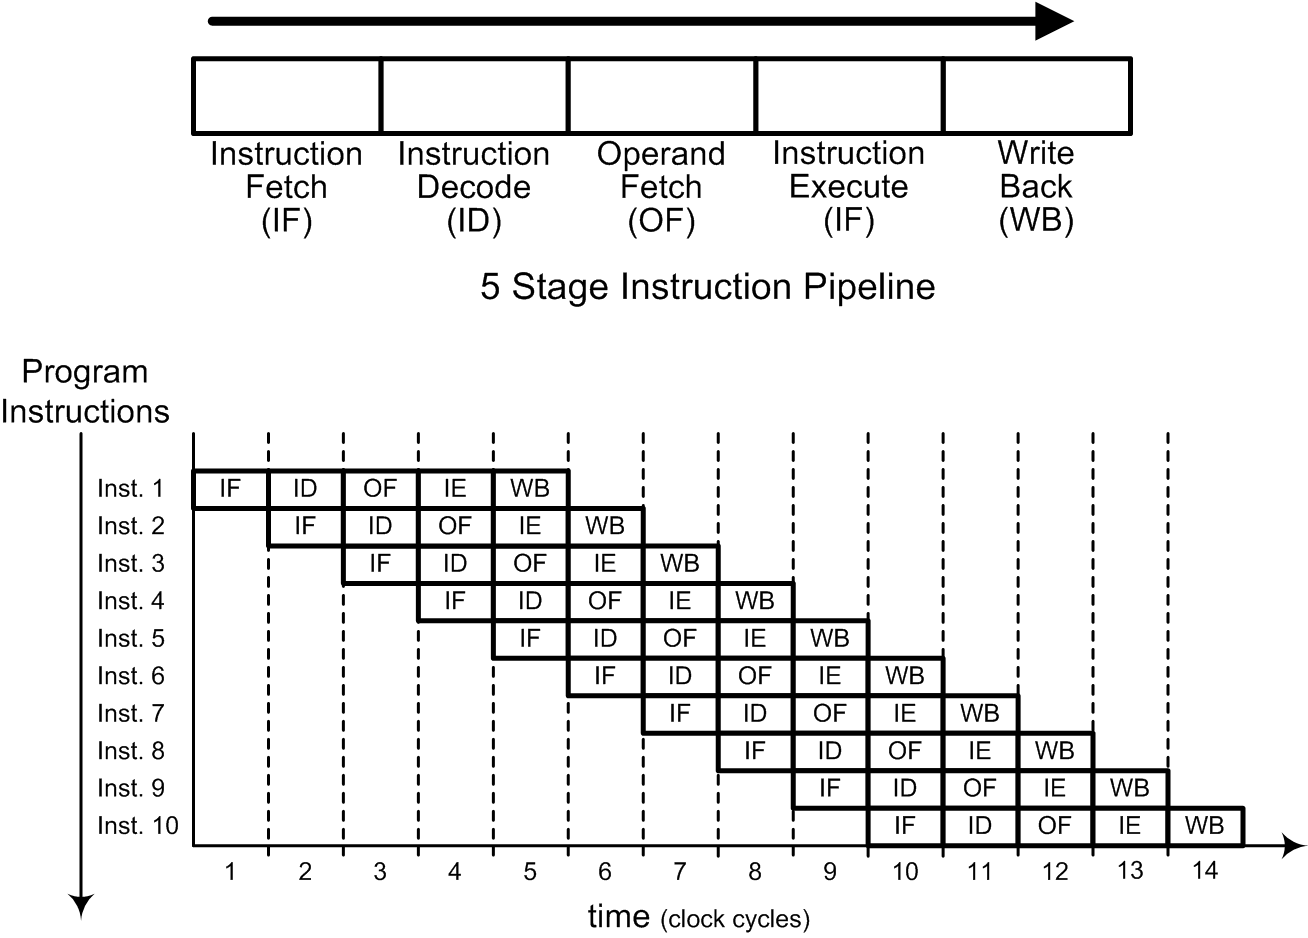
\includegraphics[width=\textwidth]{figures/pipeline2.png}
    \caption{A pipeline during execution} 
    \label{fig:pipeline}
\end{figure}

\subsubsection*{Hazards}
But pipelining is not only good, as it can cause problems when the instructions
needs to perform the same action at different times, or some data is dependent
on an earlier instruction. This can always be solved by stalling the processor, 
but it can't be done while running. To stop this, the processor must do so called 
hazard detection. When it finds that a problem will arise, it adds 'stall 
instructions', or pipeline bubbles, that basically tells the processor to stall 
for that cycle. In other words, it inserts a NOP instruction into the
pipeline.\cite{hazards-lecture}

\subsection{Optimization}

\subsubsection*{Forwarding}
Instead of inserting pipeline bubbles, forwarding can be implemented. To forward
is to send the result of an instruction back in the pipeline to an earlier
dependent step. A trivial example of this can be

\begin{verbatim}
a = 1 + 1
b = a + 1
\end{verbatim}

as \textit{b} is dependent on \textit{a}, and that instruction needs to be done.
By sending \textit{a} back, the second instruction can be completed in time.


\subsubsection*{Branch prediction}
In the case of branching, the processor can't add the next instruction to the
pipeline, as it isn't sure of what instruction is the next. To solve this
problem, branch prediction tries to guess whether or not a branch will be
followed. This allows to then find the next instruction, and thus add the next
instruction to the pipeline.


\subsubsection*{Flushing}
If a branch is taken, but was assumed not, the instruction in the pipeline must
be discarded. This is called flushing, and is done by inserting NOP instructions
instead of instructions that should be executed.
